% ============================================================================
% AI / Machine Learning contribution section -- redesigned 2026-08-15 for
% insertion into the multi-author national geosite article.
% Author of this section: EL GORRIM Mohamed (AI Research Intern, GSMI, UM6P)
% Supervised by: Dr. Ismail BEN AMAR, Sanae EL HARCHE, Mohamed EL OUALI
%
% Standalone-compilable (single-column, journal-style) excerpt intended to be
% spliced into the larger article; section/subsection numbering should be
% renumbered to fit the surrounding manuscript's structure.
%
% Every number in this section is drawn from a specific, verified source file
% in results/json/ (training/ and other/), re-derived and cross-checked
% 2026-09-01 after merging the final 722 labels that complete the dataset and fixing
% a Region-field data-quality bug in the master catalog (see git history for
% both). N grew from 939 to 1662. The classified accessibility maps
% (Figs. 3-7) are produced by 03_report_generation/make_maps.py: the deployed
% Difficult model is a Gaussian Process classifier on the Infra feature set
% (GP+Infra), and the deployed Easy model is the four-member tree ensemble
% also on the Infra feature set (Tree+Infra) -- both re-selected this pass via
% a full model-family x feature-set comparison, not assumed unchanged from
% the smaller dataset. See that script's docstring for the full
% data-provenance chain.
%
% 2026-09-01, second pass: rewritten throughout for a non-ML audience
% (geology researchers, not statisticians). Added a plain-language "How to
% Read the Numbers" section; shortened paragraphs; moved chi-square test
% statistics out of running prose into table footnotes (p-values are the
% number a reader needs to judge a claim; the test statistic behind them is
% not); gave every ML-specific term (cross-validation, p-value, precision/
% recall, AUC, the specific algorithms) a one-line plain explanation at
% first use. No numbers changed from the previous pass.
% ============================================================================
\documentclass[11pt,a4paper]{article}
\usepackage[utf8]{inputenc}
\usepackage[T1]{fontenc}
\usepackage{amsmath}
\usepackage{amssymb}
\usepackage{graphicx}
\usepackage{booktabs}
\usepackage{array}
\usepackage{multirow}
\usepackage{colortbl}
\usepackage{hyperref}
\usepackage{float}
\usepackage{geometry}
\usepackage{xcolor}
\usepackage{microtype}
\usepackage{titlesec}
\usepackage{caption}
\usepackage{enumitem}
\usepackage[numbers]{natbib}
\usepackage{newpxtext}
\usepackage{newpxmath}
\usepackage[scaled=0.90]{helvet}

\geometry{a4paper, left=25mm, right=25mm, top=25mm, bottom=28mm, footskip=12mm}
\definecolor{accent}{HTML}{2B5F72}
\definecolor{groupbg}{HTML}{EDF2F3}
\hypersetup{colorlinks=true, linkcolor=accent, citecolor=accent, urlcolor=accent}
\raggedbottom
\setlength{\parindent}{0pt}
\setlength{\parskip}{7pt}

\titleformat{\section}{\normalsize\bfseries\sffamily\color{accent}}{\thesection}{0.8em}{}
\titleformat{\subsection}{\small\bfseries\sffamily}{\thesubsection}{0.8em}{}
\titlespacing*{\section}{0pt}{14pt}{6pt}
\titlespacing*{\subsection}{0pt}{10pt}{4pt}

\captionsetup{font=small, labelfont={bf,sf}, labelsep=period}
\renewcommand{\arraystretch}{1.15}

\newcommand{\headrule}{\vspace{-2pt}{\color{accent}\rule{\linewidth}{1pt}}\vspace{4pt}}
\newcommand{\grouprow}[1]{\multicolumn{3}{@{}l}{\cellcolor{groupbg}\textbf{#1}}\\}

\newenvironment{termbox}
  {\begin{quote}\small\begin{itemize}[leftmargin=1.1em]}
  {\end{itemize}\end{quote}}

\begin{document}

% ---------------------------------------------------------------- Title ----
\begin{center}

\includegraphics[width=0.44\linewidth]{um6p_figures/um6p_gsmi_logo.png}\\[12pt]
{\color{accent!35}\rule{0.32\linewidth}{0.5pt}}\\[13pt]
{\LARGE\bfseries\sffamily Machine Learning Assessment of Geosite Accessibility in Morocco: National-Scale Application}\\[6pt]
{\normalsize EL GORRIM Mohamed$^{1}$}\\[2pt]
{\small\itshape $^{1}$Geology and Sustainable Mining Institute (GSMI), Mohammed VI Polytechnic University (UM6P)}\\[2pt]
{\small Supervised by Dr.\ Ismail BEN AMAR, Sanae EL HARCHE, Mohamed EL OUALI}
\end{center}
\headrule

\begin{abstract}
\noindent\small
Physical accessibility governs whether a geologically significant site can be turned into a geotourism or educational asset. We ask a simple question: can a computer model predict, from terrain and infrastructure data alone, how hard a geosite is to reach? We test this on 1{,}662 labeled Moroccan geosites, using a validation method designed specifically to avoid an easy but misleading way of inflating accuracy (Section~\ref{sec:reading-guide} explains why this matters and how to read every number in this paper).

At national scale, a standard model reaches 76.7\% accuracy for predicting \emph{Difficult} sites and 71.3\% for predicting \emph{Easy} sites. Once compared honestly against a "no-model-at-all" baseline, the two results tell opposite stories: the Difficult prediction is, statistically, no better than always guessing -- in fact slightly worse -- while the Easy prediction is a real, statistically confirmed improvement over guessing. Adding two new pieces of information -- each site's broad geological setting, and nearby tourism infrastructure -- measurably improves both predictions. Testing several different modeling algorithms against each other, rather than assuming the first one chosen is best, also paid off: a different algorithm (a Gaussian Process classifier, explained in Section~\ref{sec:models-compared}) turns out to be significantly better than our original choice for the Difficult prediction specifically, while our original choice remains the better one for Easy. The two prediction maps in this paper therefore come from two different algorithms, chosen because the evidence supported it, not by default.

A separate model answers a different, related question: not how hard a known geosite is to reach, but where new, not-yet-catalogued geosites are likely to be found. This "favorability" model performs very well (a discrimination score of 0.956 out of a possible 1.0). We also report, honestly, how often each accessibility model can commit to a confident answer versus when it should be treated as unreliable: roughly seven predictions in ten are trustworthy for Difficult sites, and roughly one in two for Easy sites -- the rest deserve a field check before being relied upon. A detailed, region-by-region version of this analysis is the subject of a companion paper; here we focus on the national picture and compare our approach to two other published accessibility studies.
\end{abstract}

% ==========================================================================
\section{Introduction}
Morocco's national geoheritage inventory includes geological formations of real scientific and educational value. Many of them are only useful for outreach, teaching, or tourism if visitors can actually reach them. For GSMI, accessibility is therefore not a side detail -- it is a precondition for turning a geosite into a usable asset. It is also a factor that varies enormously across a country with Morocco's topographic range, from flat Saharan coastal plains to the High and Middle Atlas.

This section asks whether accessibility can be predicted from terrain and infrastructure data alone, using standard statistical and machine-learning models. We report honestly where that approach succeeds, where it does not, and why -- including cases where the answer changed as more data became available.

Figure~\ref{fig:groundtruth} shows the underlying dataset on the map before any modeling: all 1{,}662 labeled geosites, colored by their true, expert-assigned accessibility class. Two patterns stand out and recur throughout this paper. First, labeled geosites cluster heavily in the Middle Atlas and Fés-Meknés corridor, where geoheritage documentation has historically been densest. Second, Difficult sites concentrate along the Rif and Middle Atlas mountain fronts, while the southern regions and Oriental are comparatively sparsely labeled. This coverage pattern directly shapes which regional results can be trusted, a point we return to in Section~\ref{sec:limits}.

\begin{figure}[H]
\centering
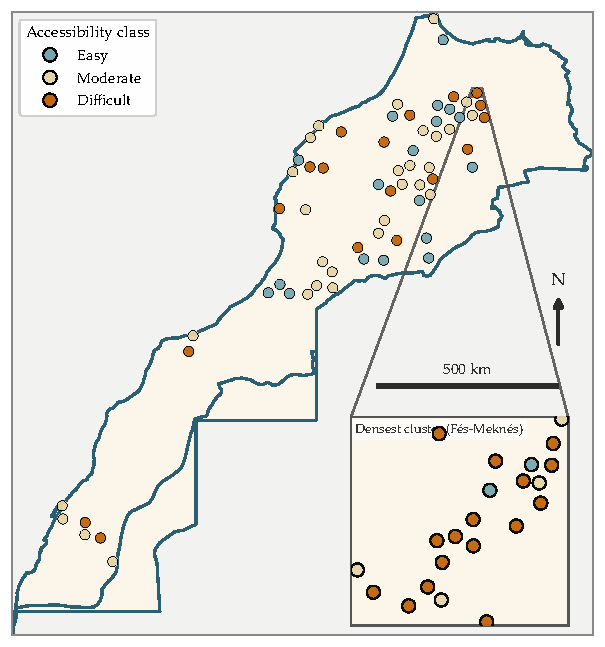
\includegraphics[width=0.82\linewidth]{figures/map_groundtruth_national.pdf}
\caption{Labeled geosites, by true accessibility class -- a spatially thinned sample is shown for legibility, with the inset magnifying the single densest cluster; all 1{,}662 sites are used throughout the analysis (Table~\ref{tab:dataset}).}
\label{fig:groundtruth}
\end{figure}

\section{How to Read the Numbers in This Paper}
\label{sec:reading-guide}
This paper reports results the way machine-learning studies conventionally do, which uses a handful of terms not common in geoscience writing. This short section defines them once, in plain language, so the rest of the paper can use them without re-explaining each time.

\begin{termbox}
\item \textbf{Accuracy} is simply the percentage of sites the model classifies correctly. On its own, a single accuracy number can be misleading (see the next point), so this paper never reports one in isolation.
\item \textbf{The majority-class baseline} is the accuracy you would get with no model at all, just by always guessing the most common label. For example, if 79\% of sites are \emph{not} Difficult, then guessing "not Difficult" every single time is already 79\% accurate -- without looking at the data once. A real model has to beat this baseline to be doing anything useful; if it does not, its accuracy figure, however large, is not evidence of learned skill.
\item \textbf{Statistical significance and $p$-values} answer the question: could this result just be luck? A $p$-value is the probability of seeing a difference this large (for instance, between a model and the majority-class baseline) purely by chance, if there were really no difference at all. Throughout this paper, we call a result \emph{significant} when $p<0.05$ -- a standard threshold across science, meaning less than a 1-in-20 chance the result is a fluke. We report the exact $p$-value every time rather than just "significant" or "not," so the reader can judge the strength of the evidence directly. The underlying statistical test used for these comparisons is McNemar's test, a standard method for comparing two classifiers evaluated on the exact same set of sites.
\item \textbf{Cross-validation} is how a model is tested fairly. Rather than checking whether the model can recite the data it was trained on, cross-validation repeatedly hides part of the data, trains on the rest, and tests only on the hidden part -- like a closed-book exam. Section~\ref{sec:validation} explains a specific and important complication for geographic data: two geosites that are very close together are, for practical purposes, the same question asked twice, and a naive test that puts one in training and the other in the test set can look artificially good without the model having learned anything real. This paper's validation protocol is built specifically to avoid that trap.
\item \textbf{Precision and recall}, for a given class such as \emph{Difficult}, answer two different questions. \emph{Precision} asks: of the sites the model flagged as Difficult, how many really are? \emph{Recall} asks: of all the sites that really are Difficult, how many did the model catch? A model can have high precision and low recall at the same time -- it is careful about calling Difficult, but as a result misses many real Difficult sites. This exact situation occurs in Section~\ref{sec:national} and is reported plainly there, not hidden behind the headline accuracy number.
\item \textbf{AUC} (Area Under the Curve) is used only for the favorability model in Section~\ref{sec:favorability}, which outputs a likelihood score rather than a yes/no label. AUC ranges from 0.5 (no better than random guessing) to 1.0 (perfect separation of true geosite locations from background terrain), and measures how well the model ranks true locations above non-locations across every possible decision threshold at once.
\item \textbf{A 95\% confidence interval} is a range around a reported number -- for instance, an accuracy of 80.8\%, [78.8, 82.6] -- that communicates how much that single number should be trusted given the sample size. It can be read as: if this whole study were repeated many times, 95\% of those repetitions would produce an accuracy somewhere in that range.
\end{termbox}

A handful of more specific technical terms -- the names of particular algorithms, and two more specialized statistical checks used once each -- are explained individually where they first appear, in Sections~\ref{sec:models-compared} and \ref{sec:calibration}.

\section{Study Area and Dataset}
The analysis covers 1{,}662 labeled geosites across Morocco's administrative regions (Table~\ref{tab:dataset}). Each site is assigned one of three accessibility classes -- \emph{Easy}, \emph{Moderate}, or \emph{Difficult} -- based on how a visitor would realistically reach it: the road type, the remaining walking distance, and the terrain along the final approach.

Every label is traceable to an external, citable source: published geoheritage and geomorphosite inventories, hiking and trail-report platforms, tourism-operator itineraries, or direct field expertise. Sites for which no independently verifiable source could be found were left unlabeled rather than guessed.

This is a single dataset, completed in three stages rather than divided into separate experimental groups: an earlier, incomplete version reached 939 labeled sites, and the current, complete version reaches all 1{,}662. 734 labels come from the original citation-traceable inventory. 206 were added in a second labeling pass (bringing the dataset to its earlier, 939-site state). 722 more were added in a third, most recent labeling pass, dated 2026-08-28, which covers nearly the entire 1{,}667-site catalog and completes the dataset at its current 1{,}662-site total. Every stage went through the same audit before use: correcting typos and non-standard region names, reassigning a site's region where its coordinates disagreed with the administrative boundary, and manually resolving every case where two labels pointed to the same coordinates but disagreed on the class.

Cross-checking the final labeling pass against the earlier, incomplete dataset surfaced ten disagreements, out of 940 sites the two had in common -- about 1\%. In every case we kept the label that had already been through the earlier audit. Three of those ten disagreements turned out to be the same same-coordinate cluster documented in an earlier audit round; the final pass also found four more cases of the same problem, this time at sites that had no previous label, so those four were excluded rather than resolved by guesswork.

Reconciling the final labeling pass against the catalog's region field also surfaced an unrelated data-quality problem: Morocco's twelve official regions were written 21 different ways across the master catalog (spelling and accent variants of the same region name). Only 8 of the 289 affected sites had ever carried a label before, which is why the problem went unnoticed until this final pass labeled the rest of them. We fixed it by matching each site's coordinates directly against the official region boundary map, which also corrected a handful of sites that had been assigned to the wrong region entirely, not just misspelled. Because of this fix, the regional totals in Table~\ref{tab:dataset} cannot be obtained by simply adding this pass's raw counts to the previously published table. Finally, an earlier practice of giving different labelers different confidence weights has been retired: every labeler's contribution is now treated equally.

\begin{table}[H]
\centering\small
\caption{Dataset composition: labeled geosites by region and accessibility class (N=1{,}662).}
\label{tab:dataset}
\renewcommand{\arraystretch}{1.15}
\begin{tabular*}{\linewidth}{@{\extracolsep{\fill}}lrrrr@{}}
\toprule
Region & Difficult & Easy & Moderate & Total \\
\midrule
Fés-Meknés & 192 & 193 & 152 & 537 \\
Béni Mellal-Khénifra & 54 & 91 & 181 & 326 \\
Tanger-Tétouan-Al Hoceima & 39 & 160 & 113 & 312 \\
Drâa-Tafilalet & 27 & 86 & 57 & 170 \\
Souss-Massa & 11 & 37 & 48 & 96 \\
Marrakech-Safi & 8 & 42 & 19 & 69 \\
Rabat-Salé-Kénitra & 4 & 21 & 19 & 44 \\
Guelmim-Oued Noun & 2 & 23 & 13 & 38 \\
Eddakhla-Oued Eddahab & 8 & 3 & 23 & 34 \\
Laayoune-Sakia El Hamra & 3 & 7 & 8 & 18 \\
Casablanca-Settat & 2 & 6 & 6 & 14 \\
Oriental & 0 & 2 & 2 & 4 \\
\midrule
\textbf{Total} & \textbf{350} & \textbf{671} & \textbf{641} & \textbf{1{,}662} \\
\bottomrule
\end{tabular*}
\end{table}

Every region grew substantially in this update. Fés-Meknés went from 337 to 537 labeled sites, Tanger-Tétouan-Al Hoceima from 128 to 312, and Béni Mellal-Khénifra from 174 to 326. Oriental, which previously had no labels at all, now has 4 (2 Easy, 2 Moderate, still none Difficult).

A few regions remain thin in one or more classes: Casablanca-Settat has only 14 labeled sites in total, Oriental has 4, and Laayoune-Sakia El Hamra has 18. This is a real, identifiable limit on which regions can support their own reliable region-specific model, even though all of these sites still contribute to the pooled national models reported here. We return to this point directly in Section~\ref{sec:limits} rather than leaving it implicit.

\section{Methodology}

\subsection{Predictor Variables}
Six terrain and infrastructure variables form the common starting feature set for every model in this study (Table~\ref{tab:variables}). Section~\ref{sec:national} adds two further pieces of information on top of this starting set -- each site's broad geological setting, and nearby tourism infrastructure -- and the models actually deployed and mapped in this paper use that expanded set, not the plain six-variable version alone.

\begin{table}[H]
\centering\small
\caption{Predictor variables used in all models, grouped by physical meaning.}
\label{tab:variables}
\begin{tabular}{@{}p{3.8cm}p{8.2cm}p{2.9cm}@{}}
\toprule
Variable & Description & Source \\
\midrule
\rowcolor{groupbg} \multicolumn{3}{@{}l}{\textbf{Terrain factors} -- what the ground itself is like at the site} \\
Slope (degrees) & Local terrain slope at the site & Copernicus DEM \\
Ruggedness & Terrain ruggedness (elevation variability in the surrounding window) & Copernicus DEM \\
Elevation (m) & Site elevation above sea level & Copernicus DEM \\
\midrule
\rowcolor{groupbg} \multicolumn{3}{@{}l}{\textbf{Infrastructure \& land cover} -- what stands between a visitor and the site} \\
Dist.\ to highway (m) & Distance to the nearest paved road segment & OSM road network \\
Dist.\ to settlement (m) & Distance to the nearest village/settlement point & OSM place points \\
LULC friction & Land-cover-based movement resistance coefficient & ESA WorldCover \\
\bottomrule
\end{tabular}
\end{table}

\subsection{Labeling Protocol}
Each site's accessibility class reflects how a visitor would reach it in practice: the road type and condition up to the nearest drivable point, and the terrain difficulty of any remaining walk on foot.

Every label carries a traceable source and a confidence level (High, Medium, or Low). Confidence was assigned by cross-checking each candidate description from the literature against independently measured road-distance data. This step specifically catches two recurring problems: a source describing a real place but at the wrong coordinates, and a source describing a different, similarly-named place elsewhere in the region.

This three-class scheme, and the accessibility reasoning behind it, follows established geoheritage-assessment practice -- specifically the accessibility-grading methodology of Mikhailenko et al.~\citep{mikhailenko2021} and the broader geoheritage assessment framework of Reynard and Brilha~\citep{reynardbrilha2017}.

\subsection{Validation Strategy}
\label{sec:validation}
Two geosites a few hundred meters apart are, for practical purposes, the same access problem: same road, same approach, same difficulty. If such near-duplicate pairs are split across training and test sets by an ordinary random split, a model can score well simply by recognizing a site it has effectively already seen, without learning anything transferable about terrain or infrastructure. Figure~\ref{fig:validation} illustrates this failure mode and how we avoid it.

To prevent it, every site within 500\,m of another is grouped into a single cluster, and an entire cluster is always held out together during testing. This is formally called 500\,m haversine-clustered, leave-one-group-out cross-validation, abbreviated LOGO-cluster CV throughout this paper. Where the sample size allowed, we additionally report leave-one-region-out validation -- training on ten regions and testing on the eleventh in full -- as the strictest available test of whether a model generalizes to genuinely new geography, not just a genuinely new site.

\begin{figure}[H]
\centering
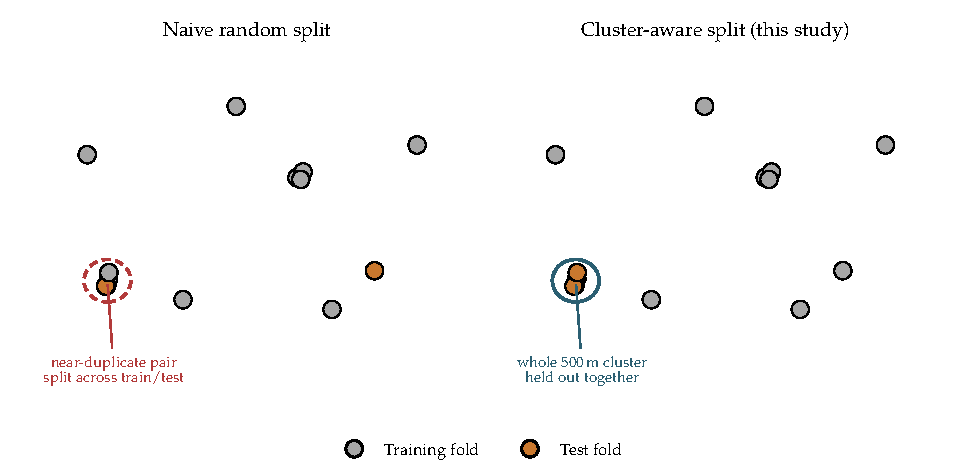
\includegraphics[width=\linewidth]{figures/validation_schematic.pdf}
\caption{Schematic illustration (synthetic points, not real data) of the two validation strategies. Left: a naive random split can place near-duplicate sites on both sides of the train/test boundary. Right: this study's cluster-aware split always keeps an entire 500\,m cluster on one side.}
\label{fig:validation}
\end{figure}

A third protocol, spatial block cross-validation, is used specifically for the geosite-location favorability model (Section~\ref{sec:favorability}). Instead of holding out clusters of near-duplicate points, it partitions the whole study area into fixed-size geographic tiles and holds entire tiles out. This model's presence/background design produces much denser, more spatially continuous point coverage than the accessibility labels, and block CV is the standard, better-suited way to test whether such a model has learned genuine geological structure rather than fine-grained spatial autocorrelation. Table~\ref{tab:cv-protocols} summarizes which protocol backs which result in this paper -- the three are not interchangeable, each answers a different robustness question.

\begin{table}[H]
\centering\small
\caption{Cross-validation protocols used in this paper, what each one tests, and where it is applied.}
\label{tab:cv-protocols}
\begin{tabular}{@{}>{\raggedright\arraybackslash}p{3.1cm}>{\raggedright\arraybackslash}p{6.2cm}>{\raggedright\arraybackslash}p{5.6cm}@{}}
\toprule
Protocol & What it tests & Used for \\
\midrule
LOGO-cluster CV & Near-duplicate sites never split across train/test & All binary and 3-class results (Section~4) \\
Leave-region-out & Generalization to a region with zero training data & Companion regional paper \\
Spatial block CV & Robustness to spatial autocorrelation, on dense point coverage & Favorability model only (Section~\ref{sec:favorability}) \\
\bottomrule
\end{tabular}
\end{table}

\subsection{Models Compared}
\label{sec:models-compared}
The working default algorithm in the rest of this section is a \emph{tree ensemble}: a vote among four different tree-based algorithms (Random Forest, XGBoost, Gradient Boosting, and LightGBM), each of which makes a prediction by learning a large set of simple yes/no splitting rules on the data. The four members vote together, and the ensemble is trained with class-balance weighting, which prevents it from simply ignoring a rare class in favor of always predicting the common one.

We did not assume this was the best available choice. Three additional, structurally different algorithms were tested under the identical LOGO-cluster protocol, as a check: a linear baseline (logistic regression, the simplest standard classifier), $k$-nearest-neighbors (which classifies a site by looking at its most similar neighbors in the data), and a Gaussian Process classifier (a more flexible, probability-based algorithm well suited to smaller datasets). One disclosed exception: the Gaussian Process's training cost grows very quickly with sample size, so instead of the full LOGO-cluster protocol (1{,}391 individual folds, impractically many for this algorithm) it was evaluated with a 10-fold cross-validation that still respects the same near-duplicate-site grouping. Table~\ref{tab:model-family} reports the resulting accuracies.

\begin{table}[H]
\centering\small
\caption{Model-family comparison, N=1{,}662, six-feature baseline, same 500\,m LOGO-cluster protocol (Gaussian Process: 10-fold group CV, see text). Best $k$ for $k$-NN chosen by LOGO-cluster accuracy among $k\in\{5,10,15,25\}$. \textbf{Bold} marks the best accuracy in each column.}
\label{tab:model-family}
\begin{tabular}{@{}lrr@{}}
\toprule
Model & Difficult acc.\ (\%) & Easy acc.\ (\%) \\
\midrule
Tree ensemble & 76.7 & \textbf{71.3} \\
Logistic Regression & 68.9 & 66.1 \\
$k$-NN ($k=10$ Diff., $k=25$ Easy) & \textbf{79.7} & 68.7 \\
Gaussian Process & 79.2 & 69.9 \\
\bottomrule
\end{tabular}
\end{table}

A raw accuracy difference is not enough to say one algorithm is really better than another -- the same significance testing described in Section~\ref{sec:reading-guide} applies here too, comparing each alternative against the tree ensemble on the identical set of sites. For the Difficult target, both $k$-NN and the Gaussian Process turn out to significantly beat the tree ensemble ($p=0.0011$ and $p=0.0073$ respectively). For the Easy target the result flips: the tree ensemble significantly beats $k$-NN ($p=0.0003$), while the Gaussian Process shows no significant difference ($p=0.173$, and carries the same 10-fold-versus-full-LOGO caveat noted above). The linear baseline trails clearly on both targets and is not considered further.

This is a genuine, evidence-driven finding, not a foregone conclusion: for the Difficult target specifically, a different algorithm really is better. Section~\ref{sec:model-choice-revisited} checks whether this conclusion still holds once the improved feature sets from Section~\ref{sec:national} are also given to these alternative algorithms, and only then settles on which model is actually deployed -- deliberately not decided here, since a better feature set could in principle change which comparison matters. (A separate, five-member variant that additionally includes an algorithm called CatBoost was used only for an internal sensitivity check, reported in the companion regional-comparison paper; it does not appear in any headline result in this paper.)

\textbf{Why did this reverse the earlier conclusion?} The identical comparison, run on the dataset's earlier, incomplete state (939 labeled sites), had found no algorithm displacing the tree ensemble -- there, the tree ensemble already ties the local majority exactly for Difficult (73.4\%), with $k$-NN and the Gaussian Process only narrowly ahead (75.3\% and 74.6\%). Splitting today's predictions by whether a site was already labeled at that earlier, 939-site stage or was added since shows the reversal is concentrated almost entirely in the 722 sites added to complete the dataset: there, the tree ensemble reaches only 80.9\% against a much higher local majority of 86.2\% (these newly-completed sites are far less Difficult-heavy, 13.9\% versus 26.6\% among the sites labeled earlier). The tree ensemble predicts Difficult for 138 of these 722 sites when only 100 actually are -- a false-alarm rate traced to the same mechanism documented in the regional companion paper's robustness section: Fés-Meknés historically supplied a disproportionate share of Difficult-labeled examples, and the tree ensemble's one global decision threshold, implicitly shaped by that region's unusually high local rate, keeps firing on genuinely easier mountain-terrain sites elsewhere. $k$-NN and the Gaussian Process classify a site by its closest neighbors in feature space rather than applying one global rule, so they track these newly-completed sites' true, much lower rate far more closely (77 and 78 predicted positive) and are not fooled the same way. Figure~\ref{fig:treevknn-mechanism} shows where this happens geographically: of the 53 newly-completed sites the tree ensemble gets wrong here but $k$-NN gets right, 42 (79\%) sit in just two mountain-terrain regions, Béni Mellal-Khénifra and Fés-Meknés -- terrain that resembles Fés-Meknés' Difficult profile closely enough to trigger the tree ensemble's rule, without the sites actually being Difficult.

\begin{figure}[H]
\centering
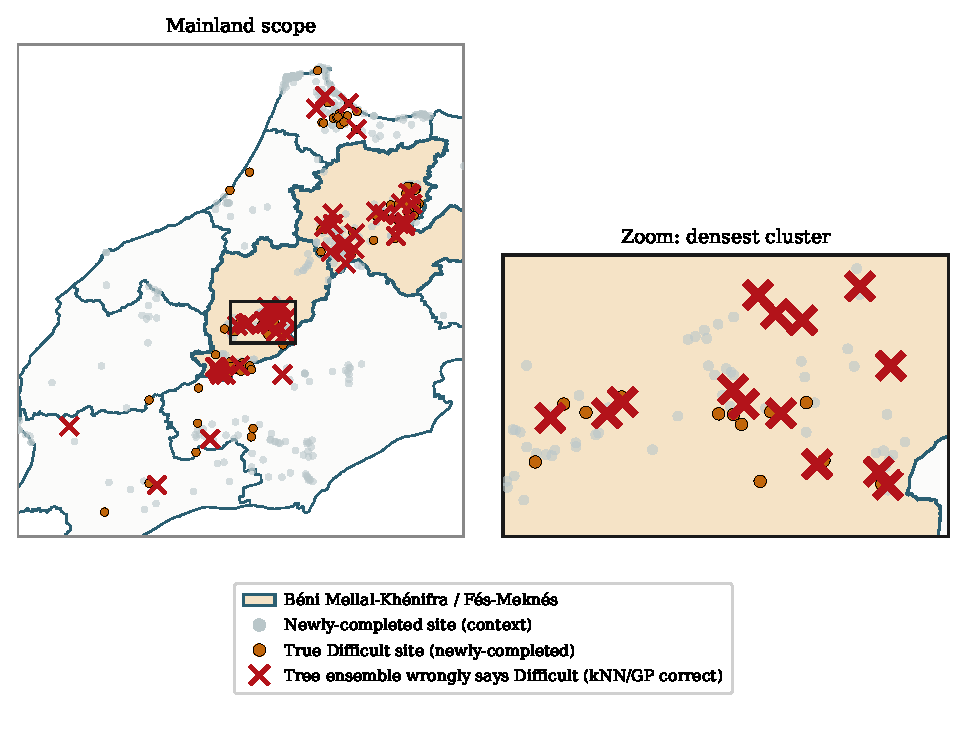
\includegraphics[width=0.92\linewidth]{figures/map_treevknn_mechanism.pdf}
\caption{The 722 sites added to complete the dataset (939$\to$1{,}662), Difficult target. Small grey dots: these newly-completed sites. Orange dots: sites genuinely Difficult. Red crosses: sites the tree ensemble wrongly predicts Difficult for, which $k$-NN and the Gaussian Process correctly predict not-Difficult. Left: 50 of the 53 crosses, cropped to where they actually occur (the remaining 3, in the far-south Guelmim-Oued Noun, Laâyoune-Sakia El Hamra, and Eddakhla-Oued Eddahab regions, fall outside this view). Right: zoom on the single densest cluster (boxed on the left), inside Béni Mellal-Khénifra -- 42 of 53 crosses overall (79\%) fall inside Béni Mellal-Khénifra or Fés-Meknés (shaded on the left).}
\label{fig:treevknn-mechanism}
\end{figure}

A parallel, opposite-direction shift explains why the tree ensemble's edge on Easy did not disappear. The newly-completed sites are much more Easy-heavy (51.9\% Easy, versus 31.5\% among the sites labeled earlier), and on exactly these new sites the tree ensemble captures that shift better than the alternatives do (71.5\% versus 65.2\% for $k$-NN and 69.1\% for the Gaussian Process). A direct check of local neighbor consistency confirms why the two distance-based methods respond in opposite directions on the two targets: completing the dataset makes an already-labeled site's nearest neighbors in feature space \emph{more} likely to share its true Difficult-vs-not label (a same-label match rate rising from 68.2\% to 69.4\%), but \emph{less} likely to share its true Easy-vs-not label (falling from 65.7\% to 62.1\%). $k$-NN and the Gaussian Process both classify a site largely by consulting its neighbors, so they benefit when neighbors get more consistent and suffer when neighbors get less consistent; the tree ensemble's global, rule-based partitions are far less sensitive to this local shift in either direction, which is exactly why it holds steady on Easy while the others slip.

\subsection{Three-Way Decision Rule}
\label{sec:decision-rule}
An alternative approach to the two-classifier setup above is to train a single model that directly predicts all three classes (Easy, Moderate, Difficult) at once. This direct approach was tried early in this project, on a smaller dataset, and set aside because it underperformed and was harder to interpret than the two-classifier approach. We revisited the comparison as the dataset grew, rather than assuming the earlier conclusion still held.

On an intermediate, smaller version of the dataset, the direct three-class model actually pulled ahead. At the current, full dataset, re-run again rather than assumed settled, the result reverses back: the direct three-class model reaches 53.4\% accuracy (against a no-model baseline of 40.4\%), while two different ways of combining the two separate classifiers reach 53.9\% and 53.4\%. All three numbers now sit within half a percentage point of each other, and a direct statistical comparison confirms they are not meaningfully different ($p=0.946$).

This back-and-forth is itself worth reporting plainly: neither approach has a durable, dataset-independent advantage over the other. The choice between them should be made on interpretability grounds -- the two-classifier approach makes it easy to state exactly why a site was labeled a given way -- rather than chasing a small, unstable accuracy difference. Table~\ref{tab:3class-confusion} shows the full breakdown of correct and incorrect predictions for the direct three-class model.

\begin{table}[H]
\centering\small
\caption{Direct 3-class model confusion matrix, N=1{,}662, 500\,m LOGO-cluster CV (rows = true class, columns = predicted). \textbf{Bold} marks correct predictions (true class = predicted class).}
\label{tab:3class-confusion}
\begin{tabular}{@{}lrrr@{}}
\toprule
 & Pred.\ Easy & Pred.\ Moderate & Pred.\ Difficult \\
\midrule
True Easy & \textbf{428} & 174 & 69 \\
True Moderate & 195 & \textbf{273} & 173 \\
True Difficult & 50 & 114 & \textbf{186} \\
\bottomrule
\end{tabular}
\end{table}

Reading Table~\ref{tab:3class-confusion} by row, the model correctly identifies 63.8\% of true Easy sites, 42.6\% of true Moderate sites, and 53.1\% of true Difficult sites. Moderate is now the hardest class to identify correctly -- a different pattern from the two-classifier framing, where Difficult specifically lags (Section~\ref{sec:national}). This plausibly reflects Moderate's role as the "everything else" middle class: once Easy and Difficult sites are both pulled apart more successfully at this larger sample size, what remains in Moderate is the harder-to-separate residual.

None of this three-class analysis is used for the headline results in Section~4, which remain this paper's primary, comparable results throughout. It is reported here as a distinct, complementary finding, not a replacement. Every headline accuracy figure elsewhere in this paper comes from a binary classifier -- Difficult-vs-not or Easy-vs-not -- each trained and validated independently against real ground truth.

The practical three-way label used operationally for those results is a simple rule, not a third trained model: a site is labeled Difficult if the Difficult-vs-not classifier flags it; Easy if the Easy-vs-not classifier flags it and Difficult did not; and Moderate otherwise. In other words, Moderate means "neither of the other two classifiers claimed this site." This rule reaches 53.9\% accuracy, essentially matching the direct three-class and ordinal-combination numbers above.

We also tested a more principled alternative, an \emph{ordinal combination}, which treats Easy, Moderate, and Difficult as points on an ordered scale and computes the Moderate probability directly from the other two:
\begin{equation}
P(\text{Moderate}) = 1 - P(\text{Easy}) - P(\text{Difficult})
\end{equation}
(clipped to stay within $[0,1]$ and renormalized before picking the most likely class). This was tested specifically to check how often the two independent classifiers disagree in a logically inconsistent way -- both flagging a site as Difficult and Easy at once. That happened for only 9 of 1{,}662 sites (0.5\%), so the more principled ordinal rule changes overall accuracy only slightly (53.4\% versus 53.9\%) despite resolving those inconsistent cases correctly.

\section{Results}
This paper reports results at national scale only. Per-region deep dives and a full cross-region comparison are the dedicated subject of a companion paper, using the same underlying dataset and methodology. Table~\ref{tab:headline} gives the headline national-scale numbers as an overview before the detailed discussion that follows.

\begin{table}[H]
\centering\small
\caption{Headline results overview: model/task, sample size, validation protocol, evaluation metric, value, and 95\% confidence interval.}
\label{tab:headline}
\renewcommand{\arraystretch}{1.3}
\begin{tabular}{@{}lrlrrr@{}}
\toprule
Model & $N$ & Validation & Metric & Value (\%) & 95\% CI \\
\midrule
Favorability & 1{,}667 & Spatial block CV & AUC & 95.6 & -- \\
Difficult (GP+Infra) & 1{,}662 & LOGO-cluster CV & Accuracy & 80.8 & [78.8, 82.6] \\
Easy (Tree+Infra) & 1{,}662 & LOGO-cluster CV & Accuracy & 73.5 & [71.3, 75.5] \\
3-class (direct) & 1{,}662 & LOGO-cluster CV & Accuracy & 53.4 & [51.0, 55.8] \\
\bottomrule
\end{tabular}

\vspace{2pt}
\noindent{\footnotesize Difficult and Easy are the deployed national models -- Gaussian Process on the Infra
feature set (GP+Infra) and the tree ensemble on the Infra feature set (Tree+Infra), respectively
(Section~\ref{sec:model-choice-revisited}). CIs are Wilson score intervals, a standard way of computing a
confidence interval for a proportion such as accuracy; not computed for the AUC row, since AUC is not a
simple proportion and would need a different (bootstrap-based) method.}
\end{table}

\subsection{National Binary Classifiers}
\label{sec:national}
At national scale, pooling all twelve labeled regions together ($n=1{,}662$), the six-feature tree-ensemble baseline reaches 76.7\% accuracy for Difficult and 71.3\% for Easy. As defined in Section~\ref{sec:decision-rule}, the two are combined operationally by exclusion: not-Difficult and not-Easy together mean Moderate.

These figures are close to the previous, smaller-sample results (74.9\% and 71.7\%). But a raw percentage-point comparison is not the right way to judge them, because the no-model baseline they are compared against also moved as the dataset grew. Difficult sites now make up a smaller share of the labeled set than before (21.1\%, down from 26.6\%), which pushes the "always guess not-Difficult" baseline up to 78.9\%. Easy sites now make up a larger share (40.4\%, up from 31.4\%), which pulls the "always guess not-Easy" baseline down to 59.6\%.

Testing both classifiers against their respective baselines gives a clear, if uncomfortable, answer for Difficult: $p=0.039$, meaning the Difficult classifier is significantly \emph{worse} than simply guessing "not Difficult" every time. This is a real and important finding, not one to downplay. For Easy, the result goes the other way: $p<0.001$, a highly significant improvement over guessing "not Easy." Neither of these two results reached significance at the smaller sample size -- both only became clear once enough data accumulated to tell the difference from chance. This divergence, one target genuinely struggling and the other genuinely succeeding, recurs throughout the rest of this section.

\textbf{Adding each site's broad geological setting helps the Difficult prediction, but not enough to close the gap.} We added a feature describing each site's geological domain (18 broad categories, taken from the master catalog's independent geological classification) to the six-feature baseline. For Difficult, this raises accuracy to 78.6\% and is a statistically confirmed improvement over the plain baseline model ($p=0.0034$) -- but it is still not enough to beat the "always guess not-Difficult" baseline ($p=0.778$, no significant advantage there). For Easy, the same addition raises accuracy only slightly, to 72.0\%, with no significant improvement over the plain baseline ($p=0.335$); it remains, as before, significantly better than guessing.

\textbf{Adding nearby tourism infrastructure helps both predictions, this time confirmed for each.} We added two more features: the number of OSM-tagged tourism and hospitality points within 10\,km of a site, and the type and size of the nearest settlement (city, town, village, or hamlet). Both were motivated by real field cases, documented separately, where a site's practical accessibility was clearly shaped by nearby organized tourism infrastructure in a way that straight-line road distance alone could not capture.

This addition raises Difficult accuracy to 78.6\% and Easy accuracy to 73.5\%, and both improvements are now statistically confirmed ($p=0.018$ and $p=0.016$ respectively). At the smaller sample size, only the Easy improvement had been confirmed; the Difficult improvement had fallen just short. This infrastructure feature set is, overall, at least as good as the geological-domain feature for Difficult and clearly better for Easy, so it is the one carried forward into the model-choice question in Section~\ref{sec:model-choice-revisited}.

The same infrastructure features, tested on the direct three-class model from Section~\ref{sec:decision-rule}, produced the single largest improvement found anywhere in this study: accuracy rose from 53.4\% to 58.7\%, a 5.3-percentage-point gain. Interestingly, this same addition did not help the three-class model at all in the smaller-sample version of this study -- another example, alongside the reversals already discussed, of why every result in this paper was re-checked rather than assumed to carry over.

\subsection{Revisiting Model Choice with the Improved Feature Set}
\label{sec:model-choice-revisited}
Section~\ref{sec:models-compared} found that, using only the plain six-feature baseline, $k$-NN and a Gaussian Process classifier both significantly beat the tree ensemble on Difficult, while the tree ensemble significantly beat $k$-NN on Easy. Before deciding what to actually deploy, this comparison needs to be checked again with the improved feature sets from Section~\ref{sec:national} -- it is entirely possible that $k$-NN or the Gaussian Process's advantage was specific to a weaker feature set, and either disappears or grows once given the same geological-domain and infrastructure additions.

\begin{table}[H]
\centering\small
\caption{Model-family comparison extended to the Domain and Infra feature sets, N=1{,}662. Best $k$ for $k$-NN chosen independently per cell, same protocol as Table~\ref{tab:model-family}. \textbf{Bold} marks the better of the two algorithms for each target, in each row.}
\label{tab:model-family-extended}
\begin{tabular}{@{}lrrrr@{}}
\toprule
& \multicolumn{2}{c}{Difficult acc.\ (\%)} & \multicolumn{2}{c}{Easy acc.\ (\%)} \\
Feature set & Tree ens. & Best of $k$-NN/GP & Tree ens. & Best of $k$-NN/GP \\
\midrule
Baseline & 76.7 & \textbf{79.7} ($k$-NN) & \textbf{71.3} & 69.9 (GP) \\
Domain & 78.6 & \textbf{80.9} (GP) & \textbf{72.0} & 70.8 (GP) \\
Infra & 78.6 & \textbf{80.8} (GP) & \textbf{73.5} & 70.2 (GP) \\
\bottomrule
\end{tabular}
\end{table}

The advantage does not disappear -- it holds under every feature set tested, and even grows slightly. GP+Domain (80.9\%) turns out to be the single best Difficult result found anywhere in this study, essentially tied with GP+Infra (80.8\%). Easy shows the mirror-image, equally consistent pattern: the tree ensemble beats both alternative algorithms under every feature set, and the gap grows as the features improve (73.5\% for Tree+Infra versus 70.2\% for GP+Infra). A direct statistical comparison between the two best Difficult candidates, GP+Domain and Tree+Infra, confirms the gap between them is real and not just noise ($p=0.020$).

GP+Domain is, however, not the model we actually deploy for the maps in this paper, for a practical reason. Geological domain is known only at the exact point locations of the 1{,}662 labeled (and 1{,}667 cataloged) geosites -- there is no map layer covering all of Morocco that could tell the model the geological domain at an arbitrary map pixel elsewhere. The infrastructure features used by GP+Infra, by contrast, genuinely can be computed anywhere from OpenStreetMap data. Since GP+Infra (80.8\%) is only 0.1 percentage points behind GP+Domain -- not a meaningful difference in practice -- it is the model that can actually produce a full-resolution national map, and so it is the one we deploy.

\textbf{The final models used throughout the rest of this paper, including its figures, are therefore: a Gaussian Process classifier on the infrastructure-augmented feature set for Difficult (80.8\% accuracy), and the tree ensemble on the same feature set for Easy (73.5\%).} This is a deliberately mixed choice -- a different algorithm for each target -- arrived at by testing the evidence at every step, not fixed as a single default from the start.

\begin{figure}[H]
\centering
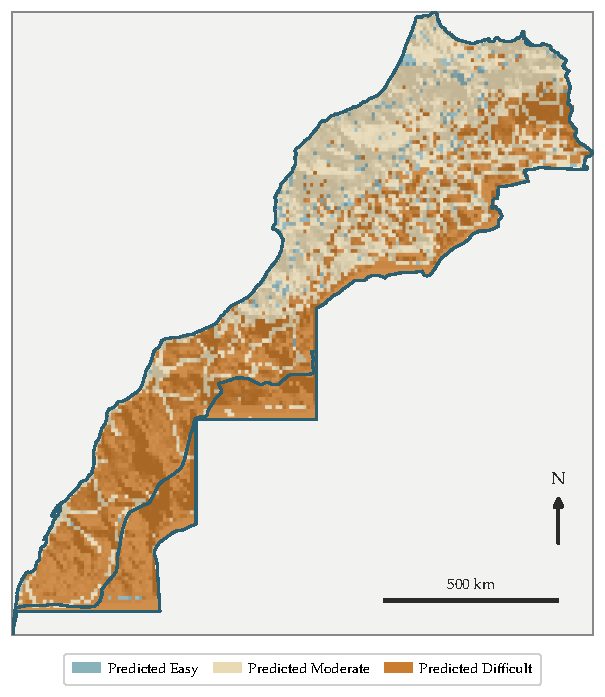
\includegraphics[width=0.68\linewidth]{figures/map_national.pdf}
\caption{National projected accessibility, all labeled regions -- Difficult layer from the deployed GP+Infra model, Easy layer from the deployed Tree+Infra model.}
\label{fig:map-national}
\end{figure}

\begin{table}[H]
\centering\small
\caption{Deployed national classifiers: precision, recall, and F1 per class (500\,m LOGO-cluster CV for Easy; 10-fold group CV for Difficult's GP component; see text), $N=1{,}662$.}
\label{tab:confusion}
\begin{tabular}{@{}llrrr@{}}
\toprule
Classifier & Class & Precision & Recall & F1 \\
\midrule
\multirow{2}{*}{Difficult vs.\ not (GP+Infra)} & Not-Difficult & 0.834 & 0.945 & 0.886 \\
 & Difficult & 0.589 & 0.294 & 0.392 \\
\midrule
\multirow{2}{*}{Easy vs.\ not (Tree+Infra)} & Not-Easy & 0.785 & 0.764 & 0.774 \\
 & Easy & 0.665 & 0.692 & 0.678 \\
\bottomrule
\end{tabular}
\end{table}

Both classifiers separate the majority class considerably better than the class of actual interest (Table~\ref{tab:confusion}). This reflects a national-scale ceiling that has appeared throughout this study: the same handful of features must now describe twelve regions with fundamentally different geology and climate at once, and the model is deliberately not told which region a site is in, to keep it usable anywhere rather than memorizing region-specific shortcuts. A pattern that looks clean within a single region individually becomes genuinely harder and more mixed once every region is pooled together. The detailed, region-by-region picture is the dedicated subject of the companion regional paper.

The deployed Difficult model's headline 80.8\% accuracy is worth unpacking, because it hides a real asymmetry. It reaches that figure by being conservative: of all the sites that are genuinely Difficult, it only catches 29.4\% of them (its recall for the Difficult class). When it does flag a site as Difficult, it is right more often than not (58.9\% precision), and it is very reliable when it says a site is \emph{not} Difficult (94.5\% recall on that much larger class). In practice, this model has learned to say "not Difficult" with confidence in most cases, and only calls Difficult on the clearest cases. That is a defensible behavior for a screening tool meant to flag likely-difficult sites for closer attention -- but it should not be read as a model that reliably catches every Difficult site nationally. The Easy model shows no such imbalance: its precision and recall are both close to 0.7.

\subsection{Calibration and Honest Uncertainty}
\label{sec:calibration}
A single accuracy figure does not say how often the model is confidently right versus quietly guessing near a coin flip. To answer that directly, we kept every model's predicted probability for each of the 1{,}662 sites (not just its final yes/no answer), obtained fairly under the same LOGO-cluster protocol, and used them for two further checks. Both checks were run on the plain six-feature baseline classifiers from Table~\ref{tab:model-family}, since the methods involved do not depend on which algorithm produced the probabilities; we do not expect the qualitative picture to change for the final deployed models, but this has not been separately re-verified for them.

\textbf{Calibration} asks: when the model says "80\% chance this site is Difficult," is that actually right about 80\% of the time? We measured this with the expected calibration error (ECE), which is close to zero for a perfectly calibrated model. Both classifiers are only mildly miscalibrated (ECE of 0.084 for Difficult, 0.058 for Easy) and are better calibrated than the earlier, smaller-sample version of this study (0.094 and 0.093). A standard correction procedure, applied only to these same held-out probabilities, meaningfully improves the Difficult model's calibration (its Brier score -- a measure of how far predicted probabilities are from the true outcome, lower is better -- falls from 0.162 to 0.143) and leaves the Easy model's calibration roughly where it was.

\textbf{Split-conformal prediction} is a way of asking the model to say "I don't know" honestly when it is not confident, instead of forcing a single guess. Concretely, for a chosen confidence level (we use 90\%), the method returns a \emph{set} of possible classes guaranteed to contain the true class 90\% of the time, checked on data the method has never seen before -- a genuine test, not a self-fulfilling one. In practice, this set contains only one class (a confident, single-answer prediction) for 70\% of Difficult predictions and 54\% of Easy predictions; the rest honestly return "could be either," rather than a forced, unreliable guess. At the smaller sample size these two rates were close together (60\% and 62\%); they have since pulled apart in the same direction as the significance results above -- Difficult became a harder problem at this sample size, Easy an easier one.

Put plainly, this paper's real, practical claim is not a single accuracy percentage. It is closer to: for roughly seven in ten Difficult calls and about one in two Easy calls, the model gives a confident, well-calibrated answer; for the rest, it explicitly flags that a field check is warranted before relying on the prediction.

\subsection{Geosite Location Favorability}
\label{sec:favorability}
This section answers a different question from the rest of the paper: not how hard a known geosite is to reach, but where new, currently uncatalogued geosites are likely to be found. We trained a separate model to distinguish real geosite locations from randomly sampled background terrain, using the current 1{,}667-site catalog.

This catalog was itself recently expanded, from 1{,}154 to 1{,}667 sites, by adding a new supervisor-provided literature source (513 new, non-duplicate localities after coordinate checks and deduplication). This catalog expansion is entirely separate from the accessibility-labeling stages described in Section~2 -- the two grew independently, and this model's results are unaffected by the accessibility-label corrections described elsewhere in this paper.

The model reaches an AUC of \textbf{0.956} under spatial block cross-validation (Figure~\ref{fig:map-favorability}), up from 0.927 on the smaller, 1{,}154-site catalog using the identical method -- the improvement comes from having more real examples to learn from, not a different approach. On that smaller catalog, the same five terrain and geology variables alone (without any infrastructure information) already reached an AUC of 0.9075; adding distance-to-settlement and land-cover friction accounted for the further gain to 0.927. This more detailed breakdown has not yet been re-run on the larger, expanded catalog; the 0.956 figure is for the full model with all variables together. (An earlier, undocumented version of this model reported AUC 0.860, but with no saved code to reproduce it, so it is not used as a comparison point here.)

One candidate variable, distance to the nearest highway, was tested and deliberately excluded. An earlier version that included it produced a favorability map that simply traced the road network almost everywhere, rather than reflecting geological structure. This is a known bias risk in this kind of model: documented geosites are disproportionately close to roads, because that is what made them easy to document in the first place, not because the terrain there is more geologically distinctive. Distance to the nearest settlement carries a similar risk in principle, but was kept because it did not produce the same obvious artifact on the map -- a disclosed, monitored trade-off rather than a fully resolved one. Separately, whether a site's soil/geology data was missing turned out to be the model's second most informative variable overall, after the geology classification itself. This could be a genuine geological signal (undocumented geology often coincides with remote, structurally distinct terrain), or it could be a sampling-bias artifact similar to the excluded highway-distance variable -- we disclose it rather than leave it unexamined.

\begin{figure}[H]
\centering
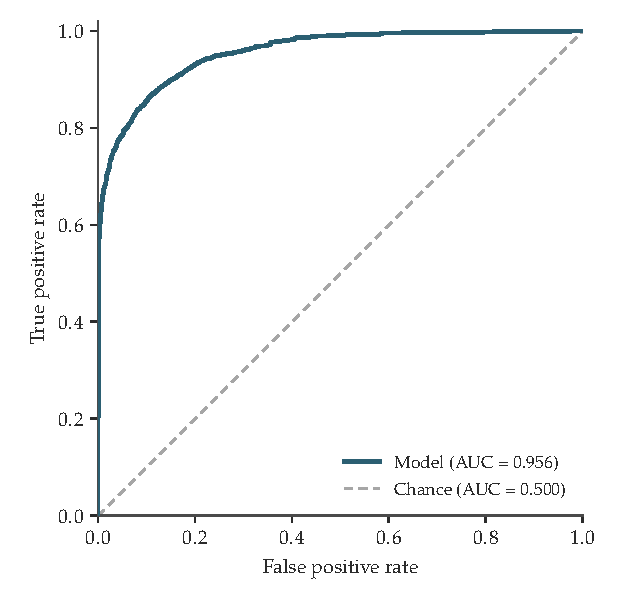
\includegraphics[width=0.42\linewidth]{figures/favorability_roc_curve.pdf}
\caption{ROC curve for the favorability model, out-of-fold predictions under the same spatial block cross-validation used to report AUC 0.956.}
\label{fig:favorability-roc}
\end{figure}

\begin{figure}[H]
\centering
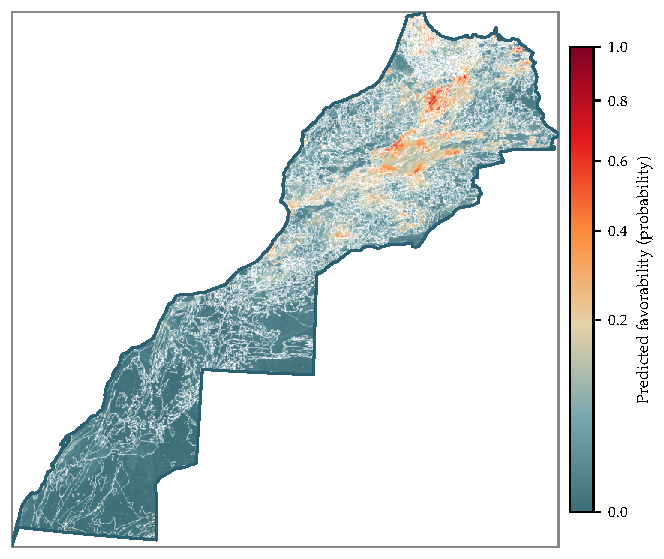
\includegraphics[width=0.68\linewidth]{figures/map_favorability.pdf}
\caption{Predicted geosite-location favorability, national extent. Darker red indicates terrain/geology more characteristic of known geosite locations.}
\label{fig:map-favorability}
\end{figure}

This favorability model's much higher discriminative power (AUC 0.956, versus the 71--81\% accuracy range for the accessibility classifiers above) makes sense given the difference in what each model is predicting. Where a geosite is likely to be is a more directly geology-driven property. How hard it is to reach additionally depends on the built road network, which is inherently noisier and more locally variable at the fixed 10--30\,m resolution used for the terrain features in this study.

\section{Related Work}
Two published studies address closely related accessibility-modeling questions and are discussed here for context, alongside the methodological reference already cited in Section~\ref{sec:validation}.

Sahani and Ghosh~\citep{sahani2021} model trail degradation risk along a 24.4\,km trail in the Sikkim Himalaya, India, using 194 point samples and seventeen conditioning factors that include directly field-measured indicators such as trail width and soil erosion. Testing logistic regression, a decision tree, and a random forest, they report 91.3--94.8\% accuracy, with logistic regression performing best -- notably the opposite ranking from our own algorithm comparison. This is plausibly explained by the difference in setting: their much smaller, single-trail study with direct field measurements likely behaves closer to a simple, linear problem than Morocco's much larger, eleven-region setting, which relies on indirect terrain proxies rather than direct field measurement.

Duran and Doğan~\citep{ardahan2026} take a fundamentally different approach for 73 candidate geosites in Ardahan Province, Türkiye. Rather than training a predictive model, they compute a deterministic accessibility index directly from network travel time, scenic visibility, and a digital-visibility score derived from Google Maps, and use it to plan optimal visitor routes. This is a complementary way of framing the same underlying problem -- calculating accessibility directly from geographic data rather than learning it from labeled examples -- and is a natural direction to explore alongside the predictive approach used here, particularly in regions with dense, reliable road-network data.

Stock et al.~\citep{stock2023} provide the methodological grounding for this study's entire validation strategy. They document how ordinary, non-spatial cross-validation systematically overestimates real-world accuracy in spatial ecological studies, for exactly the near-duplicate-site reason explained in Section~\ref{sec:validation}, and recommend block- or cluster-based validation as the fix -- the same reasoning behind the LOGO-cluster protocol used throughout this paper.

\section{Limitations and Sources of Residual Error}
\label{sec:limits}
We report five limitations explicitly below, each with a concrete, evidence-based explanation rather than a general disclaimer.

\textbf{Pooling all regions together at national scale hides regional differences, and this is likely the direct cause of the Difficult classifier's underperformance.} The national classifiers combine twelve regions of very different geology, climate, and infrastructure into one shared model, deliberately without telling the model which region a site is in (to keep the model usable anywhere, rather than memorizing region-specific shortcuts). Difficult-vs-not is now significantly worse than simply guessing at national scale (Section~\ref{sec:national}). A single pooled model cannot fully capture region-specific accessibility logic, and Difficult sites are both rare overall and unevenly spread across regions with very different terrain -- a plausible reason a single national decision boundary ends up worse than the trivial guess. Easy, by contrast, is significantly better than guessing at national scale, so pooling regions together is not universally harmful; its effect depends on which target and which feature set is used. A full region-by-region breakdown -- where the same models work well, where they do not, and why -- is the dedicated subject of the companion regional-comparison paper.

\textbf{The geological-domain feature cannot currently drive a map, which is why we deployed the infrastructure-based model instead of the marginally better domain-based one.} Geological domain is known only at the exact point locations of labeled and cataloged geosites; there is no map layer covering the whole country that would let the model look up the geological domain at an arbitrary map pixel (Section~\ref{sec:model-choice-revisited}). Domain and infrastructure features perform almost identically well for the Difficult target in table-based testing, but only the infrastructure-based model can actually produce the map figures in this paper. Building or sourcing a genuine national geological-domain map would let a future version of this work test whether the domain-based model's small advantage also holds spatially.

\textbf{Feature and framing improvements do not automatically generalize across sample sizes.} The tourism-infrastructure addition is now confirmed for both classifiers ($p=0.018$ for Difficult, $p=0.016$ for Easy); at the earlier, smaller sample size it was confirmed for Easy only. Its effect on the direct three-class model flipped even more sharply, from no measurable benefit at the smaller sample size to this study's single largest feature-addition gain at the current one. Neither a feature's statistical significance nor its effect on a particular way of framing the problem should be assumed to carry over to a different sample size or framing without re-checking -- which this study did at every step, reporting the result honestly even where it changed from an earlier finding.

\textbf{The choice of model settings (hyperparameters) is not fully separated from the final evaluation.} For each reported model, the best configuration among the available algorithms is chosen once, using the whole dataset, and then that same fixed configuration is reused across every fold of the outer evaluation that produces the headline accuracy. This is a common simplification in applied work, but it is not a fully "clean" separation between choosing the model and evaluating it: the selection step has already seen every site that later plays the role of unseen test data. For the modest, coarse settings-search used here, this typically introduces only a small optimistic bias, not a large one, but it is a real simplification and we disclose it rather than treat it as fully solved.

\textbf{Labeled coverage remains geographically and administratively uneven.} Oriental gained its first labels in this update but still has only 4 (Table~\ref{tab:dataset}); Casablanca-Settat (14) and Laayoune-Sakia El Hamra (18) also remain thin. These sample sizes are too small to support a reliable region-specific model on their own, though they still contribute usefully to the pooled national classifiers reported here. Focusing future labeling effort on these specific under-represented regions, rather than growing the dataset uniformly everywhere, would be the most efficient way to improve coverage.

\section{Conclusion}
This study applies machine learning to an independently verified, citation-traceable accessibility dataset covering 1{,}662 Moroccan geosites -- grown from an earlier, incomplete 939-site dataset to its current, complete state by adding the final labeling pass and correcting a region-assignment data-quality bug found in the process. At national scale, a plain six-feature model reaches 76.7\% accuracy for Difficult and 71.3\% for Easy.

Judged against a fair, no-model baseline, these two results tell opposite stories, both newly resolved at this larger sample size: the Difficult prediction is significantly worse than simply guessing ($p=0.039$), while the Easy prediction is significantly better ($p<0.001$). Adding two further pieces of information -- each site's broad geological setting, and nearby tourism infrastructure -- produces a statistically confirmed improvement for both targets. More importantly, re-examining which modeling algorithm works best under these improved features overturns this project's earlier conclusion: a Gaussian Process classifier is now significantly better than our original tree-ensemble choice for the Difficult target specifically ($p=0.020$), while the tree ensemble remains the better choice for Easy under every feature set tested.

The models reported and mapped throughout this paper reflect that finding directly: a Gaussian Process classifier for Difficult (80.8\% accuracy) and the tree ensemble for Easy (73.5\%), each on the infrastructure-augmented feature set -- a deliberately mixed choice, arrived at by testing the evidence rather than assumed in advance. A direct three-class model reaches 53.4\% accuracy, statistically indistinguishable from combining the two binary classifiers; both are equally valid ways of framing the same result.

Beyond accuracy, we report how much each model's predictions can actually be trusted: a confident, well-calibrated answer for roughly seven in ten Difficult predictions and about one in two Easy predictions, with an explicit recommendation to field-check the rest. A separate favorability model (AUC 0.956, on the full 1,667-site catalog) shows the same underlying feature stack also carries real signal for a related but distinct question: where currently uncatalogued geosites are likely to be found.

A full, region-by-region version of this analysis -- the natural next level of detail below these national figures -- is the dedicated subject of a companion paper. Read together with the related work discussed above, this positions the predictive approach used here as one complementary tool among several -- alongside direct field measurement and deterministic GIS-based accessibility indices -- for assessing geoheritage accessibility at national scale.

\begin{thebibliography}{9}
\bibitem{stock2023} A. Stock, E. J. Gregr, and K. M. A. Chan, ``Data leakage jeopardizes ecological applications of machine learning,'' \emph{Nature Ecology \& Evolution}, vol.\ 7, pp.\ 1743--1745, 2023.
\bibitem{sahani2021} N. Sahani and T. Ghosh, ``GIS-based spatial prediction of recreational trail susceptibility in protected area of Sikkim Himalaya using logistic regression, decision tree and random forest model,'' \emph{Ecological Informatics}, vol.\ 64, art.\ 101352, 2021.
\bibitem{ardahan2026} S. Duran and M. Doğan, ``Assessment of the Accessibility of Potential Geosites and GIS-Based Design of Optimal Georoutes in Ardahan Province (Türkiye),'' \emph{Geoheritage}, vol.\ 18, art.\ 42, 2026.
\bibitem{mikhailenko2021} A. V. Mikhailenko, D. A. Ruban, and V. A. Ermolaev, ``Accessibility of Geoheritage Sites -- A Methodological Proposal,'' \emph{Heritage}, vol.\ 4, no.\ 3, pp.\ 1080--1091, 2021.
\bibitem{reynardbrilha2017} E. Reynard and J. Brilha (Eds.), \emph{Geoheritage: Assessment, Protection, and Management}, Elsevier, Amsterdam, 2017.
\end{thebibliography}

\end{document}
